\graphicspath{{fig/sim_studies/}}

\chapter{Simulation studies}
\label{cha:sim_studies}

The feasibility of performing parameter inference on real data can be assessed by
simulation study. In simulation studies, candidate models are forward simulated for known
parameter values. This simulated data is then used to verify that the known parameter
values can be recovered by inference.

If parameter inference is \emph{not} possible on simulated data, we know that the same
inference will not be possible on real data either. Simulation studies also provide a good
opportunity to assess (and frankly, debug) our implementation of MCMC algorithms
constructed to target the posterior distribution.

\section{Global models}

Global models refer to models in which all agents take the \emph{same} parameter values.
These are in contrast to hierarchical models, in which all agents take \emph{different}
parameter values.  We shall first seek to perform simulation studies on global
models, as they represent a simpler inference problem.  

Recall from Bayes' Theorem (\cref{eq:bayes_theorem}) that to realise the posterior
distribution we need to combine the likelihood of the data with our prior beliefs. Let us
begin by considering the likelihood of observing a single agent updating its direction, in
the presence of neighbours, from $\theta_{i, t}$ to $\theta_{i, t+1}$.
From \cref{eq:students_update} we have that agent $i$ updates its direction as a draw from
the generalised Students $t$-distribution with location $\angmean{\theta}_{i,t}$, scale
$\sigma_Y$ and $\nu$ degrees of freedom. As such, the likelihood of observing this
directional update can be quantified as:
\begin{equation*}
    L(\sigma_Y, \nu, \angmean{\theta}_{i,t} \given \theta_{i,t+1}) = 
    \frac{\Gamma(\frac{\nu +1 }{2})}{\Gamma(\frac{\nu}{2})\sqrt{\pi\nu}\sigma_Y}
        \Bigg(1 + \frac{1}{\nu}
                  \bigg(\frac{\theta_{i,t+1}-\angmean{\theta}_{i,t}}{\sigma_Y}\bigg)^2
        \Bigg)^{-\frac{\nu+1}{2}},
\end{equation*}
where $\Gamma$ is the gamma function. Building on this, let us consider the likelihood of
observing agent $i$'s directions at time $t$, $t+1$ and $t+2$. As successive noise terms
are independent, we may express this likelihood as a product:
\begin{align*}
    L(\sigma_Y,\nu,\angmean{\theta}_{i,t},\angmean{\theta}_{i,t+1}\given\theta_{i,t+1},
    \theta_{i,t+2})
    = L(\sigma_Y,\nu,\angmean{\theta}_{i,t+1}\given\theta_{i,t+2})\times
    L(\sigma_Y,\nu,\angmean{\theta}_{i,t}\given\theta_{i,t+1}).
\end{align*}

In general, we wish to express the likelihood of observing agent $i$'s directional updates
over any number of times steps. Suppose then that we observe the direction of agent $i$
at time $t=1$ to $t=T$. Again, as realisations from the noise distribution are
independent, we can compute the likelihood as a product
\begin{align*}
    L(\sigma_Y, \nu, \angmean{\theta}_{i,1:T-1} \given \theta_{i,2:T})
    =& \prod_{t=1}^{T-1} L(\sigma_Y,\nu,\angmean{\theta}_{i,t} \given \theta_{i,t+1}) \\
    =& \prod_{t=1}^{T-1} 
        \frac{\Gamma(\frac{\nu +1 }{2})}{\Gamma(\frac{\nu}{2})\sqrt{\pi\nu}\sigma_Y}
        \Bigg(1 + \frac{1}{\nu}
                  \bigg(\frac{\theta_{i,t+1}-\angmean{\theta}_{i,t}}{\sigma_Y}\bigg)^2
        \Bigg)^{-\frac{\nu+1}{2}},
\end{align*}
where $\angmean{\theta}_{i,1:T-1}$ is shorthand for
$\angmean{\theta}_{i,1},\angmean{\theta}_{i,2},\ldots,\angmean{\theta}_{i,T-1}$, and
similarly for $\theta_{i,2:T}$. Finally, although we have expressed the likelihood of
observing a single agent's directional changes over $T$ observations, we really wish to
express the likelihood of observing \emph{an entire flock's} directional changes over $T$
observations. Consider observing a flock of $N$ individuals over $T$ time steps. The
likelihood of observing this data is then given by
\begin{align}
    \label{eq:likelihood}
    \begin{split}
    L(\sigma_Y, \nu, \angmean{\theta}_{1:N,1:T-1} \given\theta_{1:N,2:T}) 
    &= \prod_{i=1}^N \prod_{t=1}^{T-1} L(\sigma_Y,\nu,\angmean{\theta}_{i,t}\given\theta_{i,t+1})  \\
    &= \prod_{i=1}^N \prod_{t=1}^{T-1} 
        \frac{\Gamma(\frac{\nu +1 }{2})}{\Gamma(\frac{\nu}{2})\sqrt{\pi\nu}\sigma_Y}
        \Bigg(1 + \frac{1}{\nu}
                  \bigg(\frac{\theta_{i,t+1}-\angmean{\theta}_{i,t}}{\sigma_Y}\bigg)^2
        \Bigg)^{-\frac{\nu+1}{2}}.
    \end{split}
\end{align}

The likelihood function for all our models takes the same form. What differs
between models is the specification of the weighting function and the
corresponding computation of $\angmean{\theta}_{i,t}$.

\subsection{Vicsek model}

We simulate the movements of $N=45$ agents for $T=200$ time steps, according to the Vicsek
model. We desire to work with simulated data which is similar to real data we
study later. As such, the initial conditions for this simulation are taken from the
first frame of a real flocking event. Parameters $r=50$, $\sigma_Y=0.03$ and $\nu=7$ are
set for this simulation. \cref{fig:vicsek_sim_study} shows the data realised by this
simulation.

\begin{figure}[tb]
    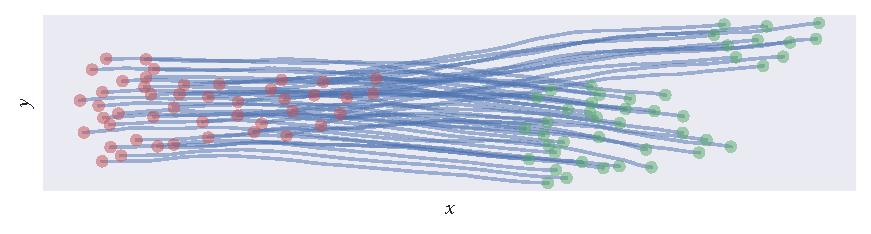
\includegraphics{vicsek_sim.pdf}
    \caption{The trajectories of $N=45$ agents simulated over $T=200$ time steps according to
    the Vicsek model. The initial conditions of the simulation reflect that of a real
flocking event. The parameters of the model are given by $r=50$, $\sigma_Y=0.03$ and
$\nu=7$.}
    \label{fig:vicsek_sim_study}
\end{figure}

The likelihood of observing this data is given by \cref{eq:likelihood}. However,
to target the posterior we also need to specify prior beliefs about the model parameters.
To allow the data to drive the inference we shall specify weakly informative prior
beliefs. Once realisations from the posterior have been made, we overlay our prior
beliefs to give an idea of how much our beliefs have updated in light of the data. 
\begin{align*}
    r           & \sim \Ga(50, 5) \\
    \sigma_Y    & \sim \Ga(2, 100)\\
    \nu         & \sim \Ga(2, 0.1)
\end{align*}

\begin{figure}[tb]
    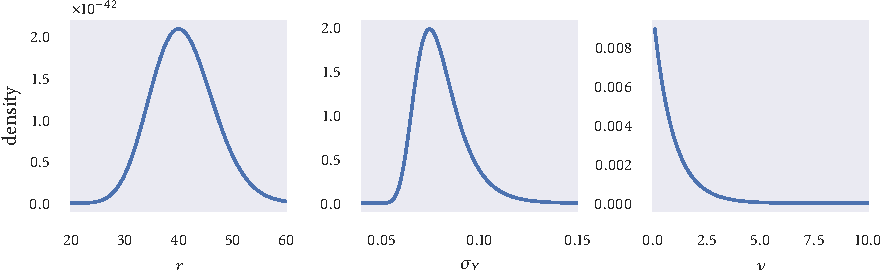
\includegraphics{priors.pdf}
    \caption{Weakly informative prior beliefs specified for the parameters of the Vicsek model.}
\end{figure}

The NUTS algorithm implemented by Stan requires a continuously differentiable posterior
distribution. Unfortunately, the discontinuity in the weighting function of the
Vicsek model results in a discontinuous posterior. As such, Stan cannot be used to infer
the parameters of this model. Instead, we shall target the posterior distribution with a
random walk Metropolis--Hastings sampler.


\subsection{Continuous models}

\subsubsection{Power-law weighted}

\subsubsection{Gaussian weighted}

\subsection{Topological model}

\section{Hierarchical models}
